\documentclass[25pt, a0paper, portrait, margin=0mm, innermargin=15mm,blockverticalspace=15mm, colspace=15mm, subcolspace=8mm]{tikzposter}

\usepackage[utf8]{inputenc}
\renewcommand{\refname}{Références}
\usepackage{lipsum} 
\usepackage{fancyhdr}
\usepackage{graphicx}
\usepackage{svg}
\usepackage{subcaption}
\usepackage[scaled]{helvet}
\usepackage{xeCJK}
\setCJKmainfont{Noto Serif CJK SC}
\renewcommand\familydefault{\sfdefault} 
\usepackage[T1]{fontenc}
\usepackage{transparent} % transparence des images

\usepackage{soulutf8} % surligner du texte
%\sethlcolor{} % couleur du surlignage

\usepackage[backend=biber,
    style=numeric-comp,
    maxcitenames=1,
    maxbibnames=1,
    %backref=true
    ]{biblatex}

\usepackage{colortbl} % colorer ligne d'un tableau
\usepackage{xspace}

\usepackage{tikz}
\usetikzlibrary{arrows,shapes}

\usepackage{enumitem} % changer les points de itemize


\tikzposterlatexaffectionproofoff %enlever phrase en bas à droite
\usetheme{Simple} %différents thèmes tikzposter

% ---- Couleurs
\definecolor{mypink1}{rgb}{0.858, 0.188, 0.478}
\definecolor{titlecolor}{RGB}{74, 114, 159}
\definecolor{titledarkcolor}{RGB}{51,102,153}
\definecolor{LightGrey}{RGB}{232, 232, 232}
\definecolor{Grey}{RGB}{222, 223, 225}
\definecolor{DarkerGrey}{RGB}{215,217,219}
\definecolor{FontColor}{RGB}{131,136,138}
\definecolor{Red}{RGB}{204,0,0}
\definecolor{L-lig}{RGB}{25,124,192}
\definecolor{point-lig}{RGB}{54,104,163}
\definecolor{G-lig}{RGB}{62,66,68}
\definecolor{Main_Blue}{RGB}{59, 122, 187}

\definecolor{Orange}{RGB}{240,163,10} 
\definecolor{Gray}{RGB}{186,200,211}
\definecolor{LightRed}{RGB}{214,98,93}
\definecolor{LightBlue}{RGB}{160,200,217}
\definecolor{LightGreen}{RGB}{130,161,119}
\definecolor{Violet}{RGB}{190,144,252}
% ----

\colorlet{blocktitlefgcolor}{point-lig} %titre des blocks
\colorlet{blocktitlebgcolor}{Grey} %couleur des lignes blocks
%\colorlet{blockbodybgcolor}{mypink1}%????
\colorlet{blockbodyfgcolor}{FontColor} %couleur du texte dans blocks
%\colorlet{innerblocktitlebgcolor}{G-lig}
\colorlet{innerblocktitlebgcolor}{L-lig}
\colorlet{innerblocktitlefgcolor}{white}
\colorlet{notefrcolor}{Red!60} % ligne autour cadre notes
\colorlet{notefgcolor}{white} % couleur police notes
\colorlet{notebgcolor}{Red!60} % BG couleur des notes


% ---- Titre
\settitle{ 
\begin{minipage}[b]{0.9\linewidth}
\vspace{2cm}
\hspace{1cm}\color{white}{ \Huge\textsc{\textbf{\@title}} \par } \vspace*{2em} \hspace{1cm}\color{white}{\LARGE \@author \par} \vspace*{2em} \hspace{1cm}{\Large \@institute}\vspace{0.5cm} \end{minipage}
\hfill
\begin{minipage}{0.2\linewidth}

%\vspace{-15cm}
%%% insert second logo at the top
% \transparent{0.6}
\includegraphics[scale=1.1]{images/Logos/logoMIAI_white.png}

%\vspace{5cm} 

% \hspace{2.2cm}\transparent{0.6}
\includegraphics[scale=1.3]{images/Logos/logo_blanc.png}
\end{minipage}}

\definetitlestyle{sampletitle}{
width=840mm, roundedcorners=0, linewidth=2pt, innersep=15pt,
titletotopverticalspace=0mm, titletoblockverticalspace=30mm
}{\begin{scope}[line width=\titlelinewidth, rounded corners=\titleroundedcorners]\draw[fill=point-lig, color=point-lig]
(\titleposleft,\titleposbottom) rectangle (\titleposright,\titlepostop);
\end{scope}}



\title{\rightline{The Course Plan of The Magic University}}
% \author{\rightline{葉珈妤、吳浩瑋、周庭碩、張惟鈞}}
\author{\rightline{Chia-yu Yeh, Hao-wei Wu, Ting-shou Chou, Wei-chun Chang}}
\institute{\rightline{Taipei Private YanPing High School}}
    
\usetitlestyle[]{sampletitle}
\setlength{\columnseprule}{0.4pt}
\addbibresource{Biblio/Biblio.bib}

%%%%%%%%%%%%%%%%%%%%%%%%%%%%%%%%%%%%%%%%%%%%%%%%%%%%%%%%%%%
\begin{document}
\maketitle 
% --- Lignes entre les colonnes
\draw[DarkerGrey, line width=2mm, loosely dotted] (0,35) -- (0,-45); 
% \draw[DarkerGrey, line width=2mm, loosely dotted] (15,35) -- (15,-40);

%------------------------------------------------------------------------------
% --------------------- CORPS DU POSTER ---------------------
\begin{columns}
\column{1}
\begin{subcolumns}
    %%%%%%%%%%%% COLONNE 1 %%%%%%%%%%%%%
    \subcolumn{.5}
   
    % ---------------------------------INTRODUCTION ----------
        \block{\textsc{Introduction}}{
            \hspace*{2cm} This poster is the opinions and answers put forward on the topic "The Course Plan of The Magic University" of the Mathematical Modeling Hackathon. The topic requires that daily courses be arranged in the nine-day curriculum of three semesters. Each course has a physical strength value and points, which represent the physical strength required to learn this class and the points that can eventually be obtained. And you are not allowed to spend more than 100 points of physical strength every day. Find the average value of this plan implemented many times and find the best course selection strategy. 

\hspace*{2cm} The following which is based on the points is our understanding of the topic and the proposed solutions .We utilize the program and compares ratios of points and physical strength values to find the average points obtained by multiple implementations of this plan.  
            \vspace{-2cm}
        }
    
    % ---------------------------------METHODS----------
        \block{\textsc{Methods}}{
            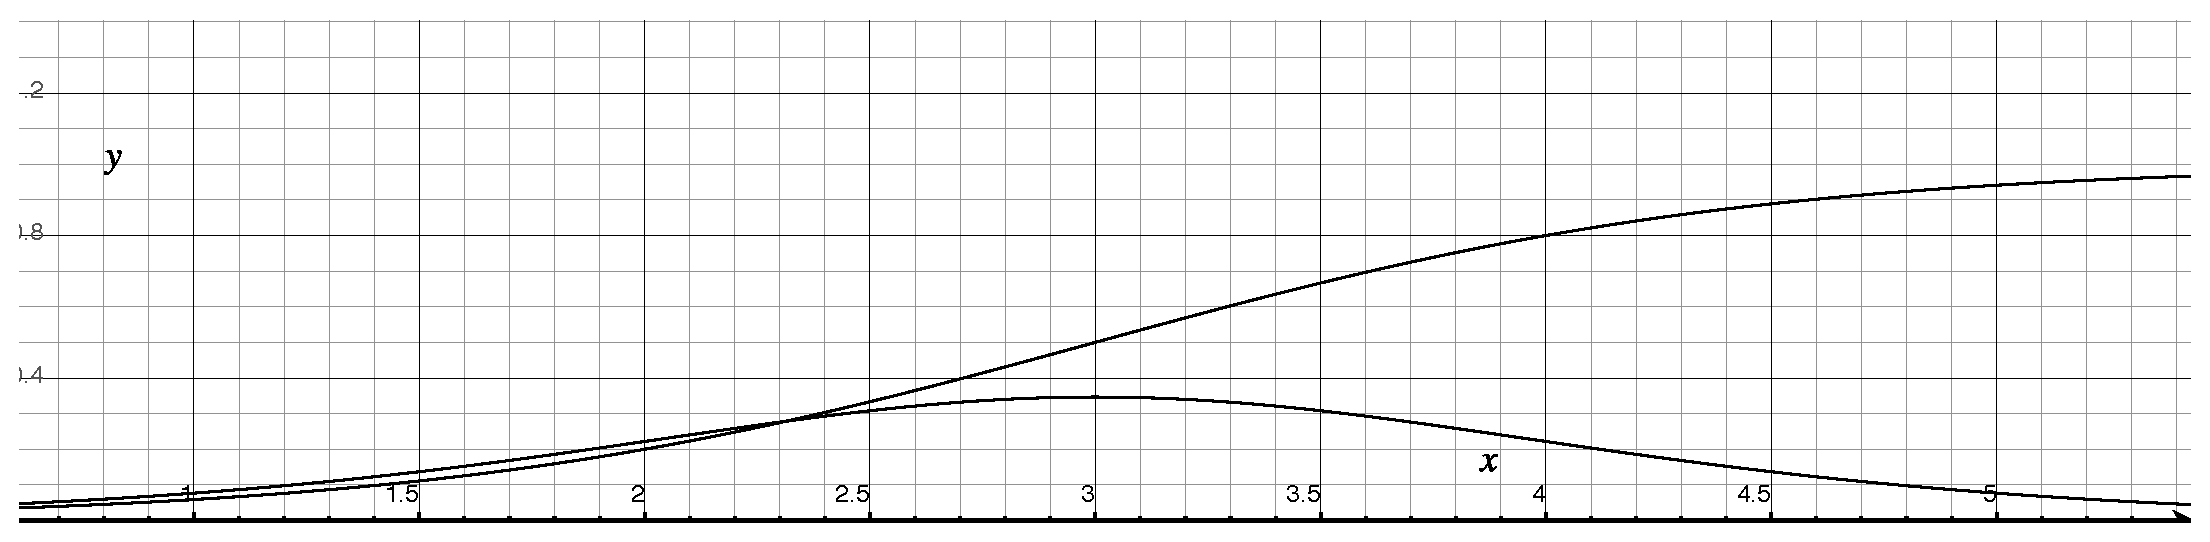
\includegraphics[scale=1.02]{images/F(x)_ext.eps}

% $f(x) = 1-\frac{1}{1+2^{2(x-3)} } $

There is an $F()$ mentioned in the title. 
The rising line in the figure above is the $Function\ F()$ curve provided by the topic, while the other is the $Function\ F$ after differential. We can know that the light color line reached the highest peak of the increase at 3. Therefore, when the second to third and third to fourth exercises are equal and the largest, to get the result of the most points in one more class, we try to set the number of single-subject exercises to 4. 
~\\

\innerblock{Expected Value}{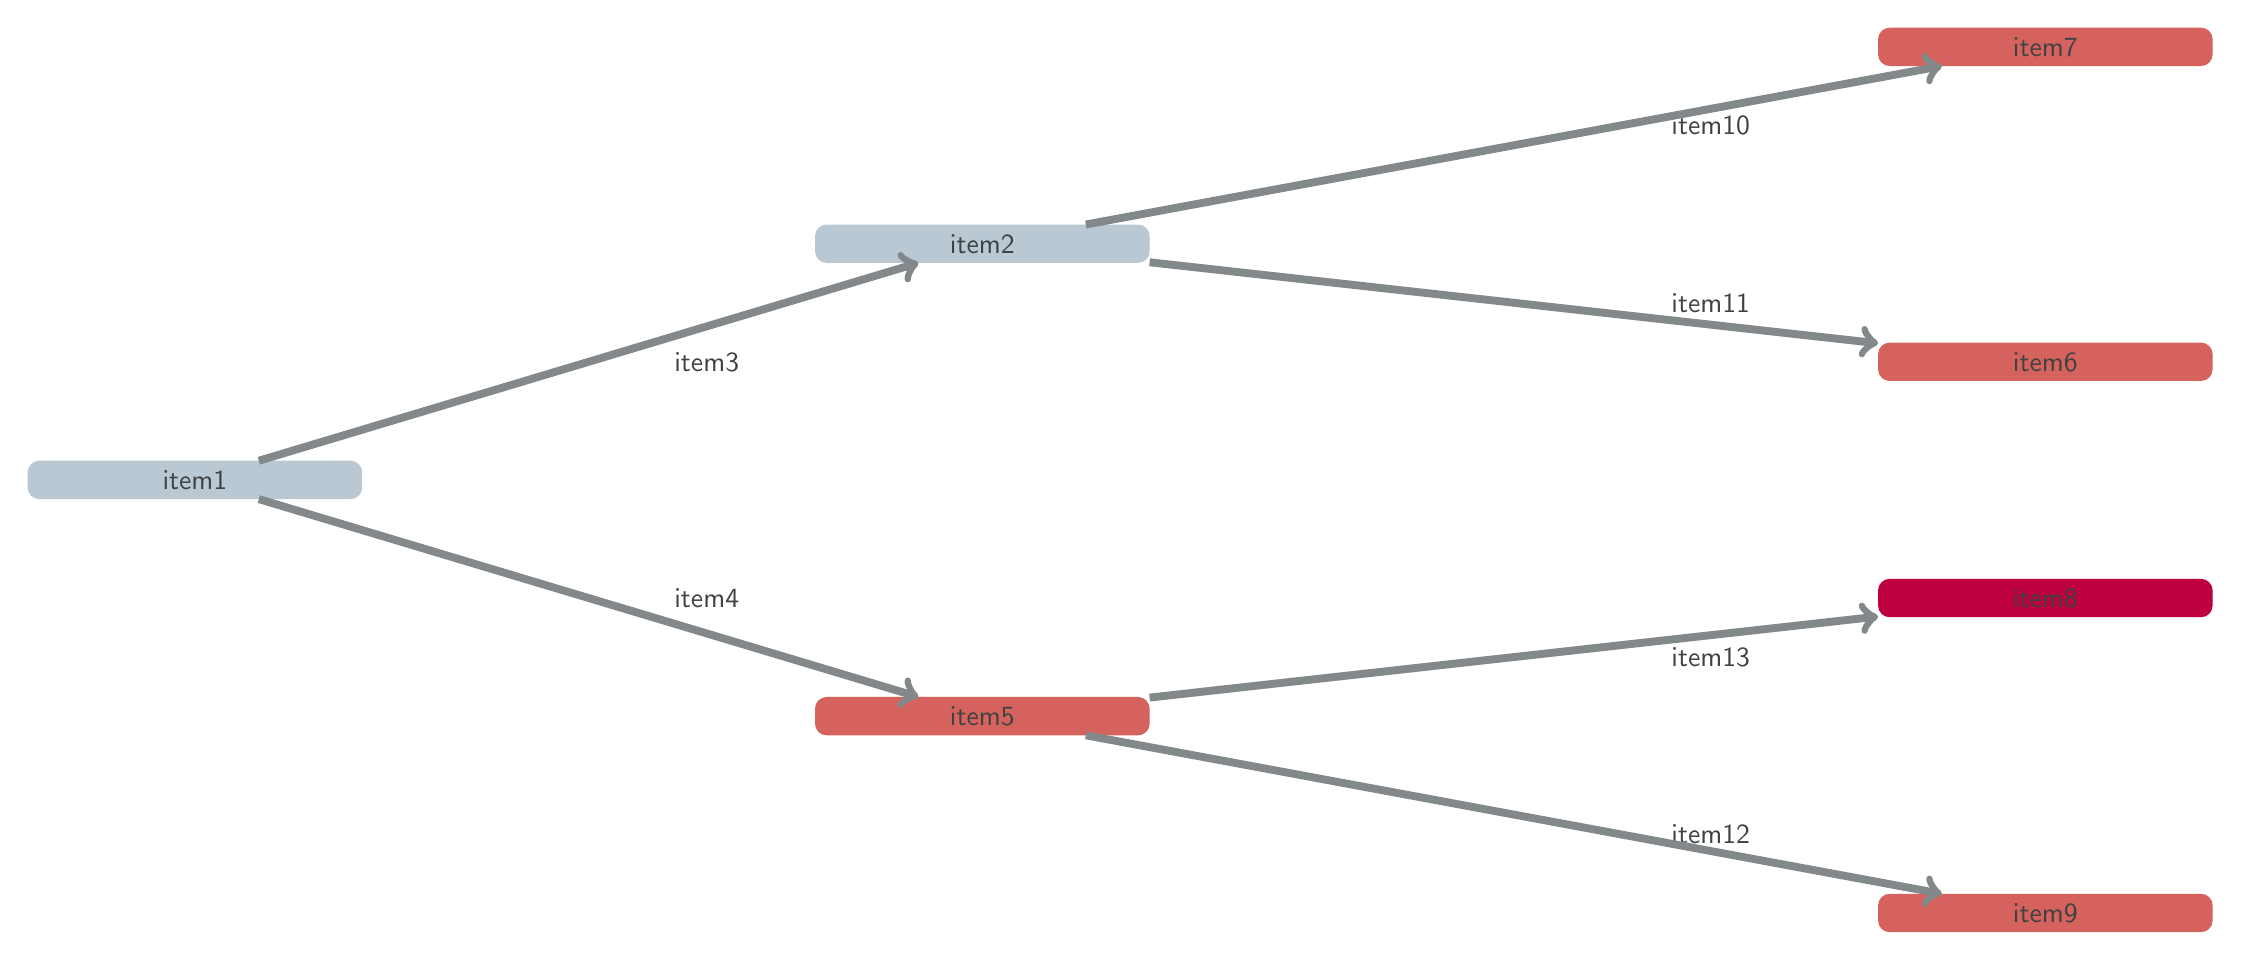
\begin{tikzpicture}
% \node[draw=Orange,fill=Orange,text=G-lig,text width=6cm, rounded corners, text centered] (item1) at (2,4) {item1};

\node[draw=Gray,fill=Gray,text=G-lig,text width=4cm,rounded corners, text centered] (item1) at (7,0) {item1};

\node[draw=Gray,text width=4cm,fill=Gray,rounded corners, text centered, text=FontColor, text=G-lig] (item2) at (17,3) {item2};

\node[text width=4cm,rounded corners, text centered, text=FontColor, text=G-lig] (item3) at (13.5,1.5) {item3};

\node[text width=4cm,rounded corners, text centered, text=FontColor, text=G-lig] (item4) at (13.5,-1.5) {item4};

\node[draw=LightRed,text width=4cm,fill=LightRed,text=G-lig,rounded corners, text centered] (item5) at (17,-3) {item5};

\node[draw=LightRed,text width=4cm,fill=LightRed,text=G-lig,rounded corners, text centered] (item6) at (30.5,1.5) {item6};

\node[draw=LightRed,text width=4cm,fill=LightRed,text=G-lig,rounded corners, text centered] (item7) at (30.5,5.5) {item7};

\node[draw=purple,text width=4cm,fill=purple,text=G-lig,rounded corners, text centered] (item8) at (30.5,-1.5) {item8};

\node[draw=LightRed,text width=4cm,fill=LightRed,text=G-lig,rounded corners, text centered] (item9) at (30.5,-5.5) {item9};

\node[text width=4cm,text=G-lig,rounded corners, text centered] (item10) at (26.25,4.5) {item10};

\node[text width=4cm,text=G-lig,rounded corners, text centered] (item11) at (26.25,2.25) {item11};

\node[text width=4cm,text=G-lig,rounded corners, text centered] (item12) at (26.25,-4.5) {item12};

\node[text width=4cm,text=G-lig,rounded corners, text centered] (item13) at (26.25,-2.25) {item13};

\draw[->,line width=1mm, draw=FontColor,] (item1) to (item2);
\draw[->,line width=1mm,draw=FontColor] (item1) to (item5);
\draw[->,line width=1mm,draw=FontColor] (item2) to (item6);
\draw[->,line width=1mm,draw=FontColor] (item2) to (item7);
\draw[->,line width=1mm,draw=FontColor] (item5) to (item8);
\draw[->,line width=1mm,draw=FontColor] (item5) to (item9);

\end{tikzpicture}

}

$ R \% \times Points \times [1 - Q\% \times(1 - K\%)] $

% \hspace{2.2cm}
% \transparent{0.6}

In terms of code, it can be implemented in a way similar to random algorithms. Specifically, we will list all possible courses for each day first, and then we can use the number to fill in each semester. Because there are many restrictions when filling the course, we will pop out the course when it doesn't meet the requirements. 
~\\

The expectation of using random as the basis for course selection is about 60. After repeating it one hundred times, it can reach the peak of 99.
~\\

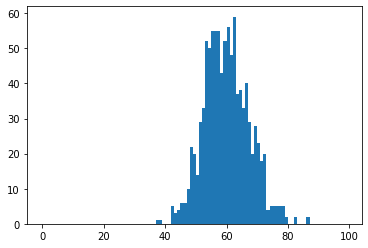
\includegraphics[scale=1.3]{images/1000times.png}
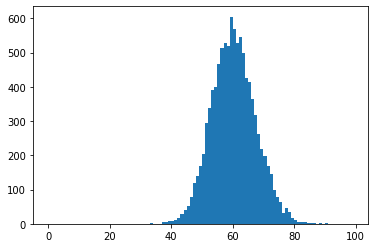
\includegraphics[scale=1.3]{images/10000times.png}

Figure 1 above shows the point distribution diagram of randomly extracting all legally selected courses 1000 times; Figure 2 shows the point distribution diagram randomly extracting 10000 times. From the two charts,  the maximum value can be found from this search, which is 95.13.
            \vspace{-2cm}
        }
    
    % --------------------------------- RESULTS ----------    
    \block{\textsc{Results}}{
                    \tikzstyle{na}=[baseline=-.25ex]
        \tikzstyle{every picture}+=[remember picture]
        \vspace{0.5cm}
        
        
        \vspace{0.5cm}
        \lipsum[1]
            
          \vspace{-2cm}
            \vspace{-2cm}
        }
          
    %%%%%%%%%%%%%%% COLONNE 2 %%%%%%%%%%%%%
    \subcolumn{.5}
    
        % ---------------------------------  PARTIE 3----------
        \block{\textsc{Partie 3}}{\innerblock{}{
        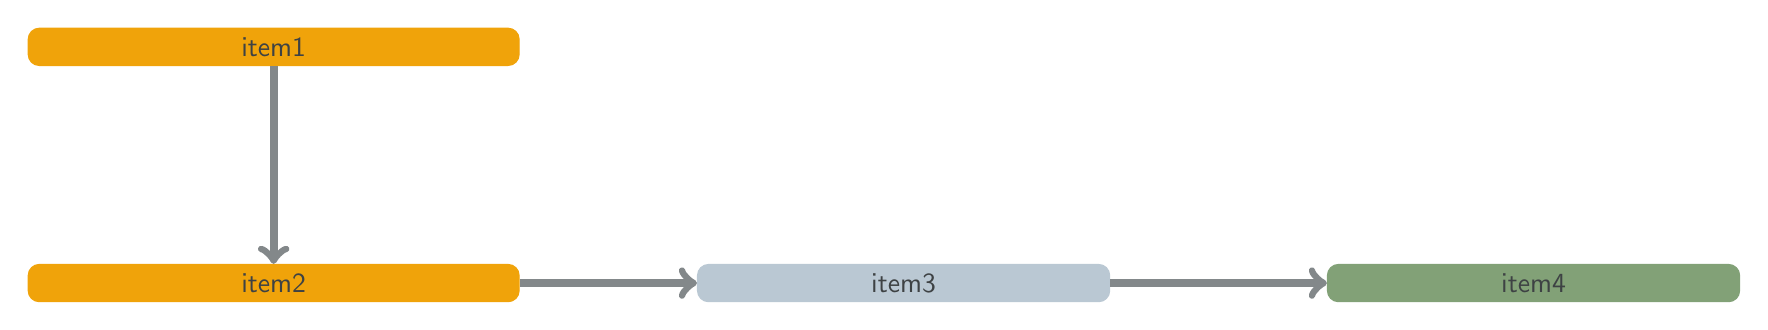
\begin{tikzpicture}
\node[draw=Orange,fill=Orange,text=G-lig,text width=6cm, rounded corners, text centered] (item1) at (2,4) {item1};

\node[draw=Orange,fill=Orange,text=G-lig,text width=6cm,rounded corners, text centered] (item2) at (2,1) {item2};

\node[draw=Gray,text width=5cm,fill=Gray,rounded corners, text centered, text=FontColor, text=G-lig] (item3) at (10,1) {item3};

\node[draw=LightGreen,text width=5cm,fill=LightGreen,text=G-lig,rounded corners, text centered] (item4) at (18,1) {item4};

\draw[->, line width=1mm, draw=FontColor] (item1) to (item2);
\draw[->,line width=1mm, draw=FontColor] (item2) to (item3);
\draw[->,line width=1mm, draw=FontColor] (item3) to (item4);

\end{tikzpicture}
} \lipsum[2]
        \vspace{-2cm}}
            
        \note[targetoffsetx = 3cm, targetoffsety = 1cm, angle = 20, connection]{\textbf{exemple de note}}

        
    % --------------------------------- PARTIE 4  ----------
        \block{\textsc{Partie 4}}{ \lipsum[3]
            \vspace{-2cm}
        }

 
    \end{subcolumns}
    

    % ---------------------------------  BIBLIO ----------
    \block{}{\vspace{1cm}
       \printbibliography}
       \end{columns}

% ----------------- Ligne colorée à la fin du document -------------
\node [above right, text=white,outer sep=45pt,minimum width=\paperwidth, align=center, draw, fill=titledarkcolor, color=point-lig] at (-43.6,-61) { \textcolor{white}{\normalsize Contact: prenom.nom@univ-grenoble-alpes.fr}};

\end{document}